\documentclass[12pt,a4paper]{article}


\fontsize{12}{14}\selectfont
\usepackage[T1]{fontenc}
\makeatletter
\title{SYSG5 : Exploitation de failles de sécurité LINUX}
\let\Title\@title
\author{Antoine Ghigny - 56359}          \let\Author\@author
\date{24/11/2022}           \let\Date\@date
\makeatother

\usepackage{titling}

\usepackage[a4paper,
            bindingoffset=0.2in,
            left=1in,
            right=1in,
            top=1in,
            bottom=1in,
            footskip=.25in]{geometry}
            
\usepackage{blindtext}
\usepackage{hyperref}
\usepackage{graphicx,color, caption}
\usepackage{epsfig}
\usepackage{fancyhdr}
\usepackage{listings}
\usepackage{color}
\usepackage{makeidx}
\usepackage{verbatim}

\graphicspath{ {./images/} }

% Valeurs par défaut le lstset
\lstset{
    language=C++,
     basicstyle=\footnotesize\ttfamily, % style par défaut 
     literate={â}{{\^a}}1 {ê}{{\^e}}1 {î}{{\^i}}1 {ô}{{\^o}}1 {û}{{\^u}}1
		 {ä}{{\"a}}1 {ë}{{\"e}}1 {ï}{{\"i}}1 {ö}{{\"o}}1 {ü}{{\"u}}1
		 {à}{{\`a}}1 {é}{{\'e}}1 {è}{{\`e}}1 {ù}{{\`u}}1 
		 {Â}{{\^A}}1 {Ê}{{\^E}}1 {Î}{{\^I}}1 {Ô}{{\^O}}1 {Û}{{\^U}}1
		 {Ä}{{\"A}}1 {Ë}{{\"E}}1 {Ï}{{\"I}}1 {Ö}{{\"O}}1 {Ü}{{\"U}}1
		 {À}{{\`A}}1 {É}{{\'E}}1 {È}{{\`E}}1 {Ù}{{\`U}}1,
    morekeywords={pipe,fork,strstr,close,fprintf,fopen,system,mkdir,perror,stat,fclose, puts, read, exit, open, exit, clear, echo, rm, make, id}, % ajoute des mots-clés supplémentaires
    commentstyle=\color[rgb]{0.133,0.545,0.133}, % style des mots-clés : vert foncé
    keywordstyle=\color[rgb]{0.737,0.051,0.051}, % style des commentaires : rouge foncé
    stringstyle=\color[rgb]{0.627,0.126,0.941}, % style des chaînes de caractères : violet
    numberstyle=\tiny, % style des numéros de ligne : petit
    numbersep=5pt, % espace entre le code et les numéros de ligne
    backgroundcolor=\color[rgb]{0.95,0.95,0.95}, % couleur de fond : gris clair
    frame=single, % ajoute un cadre autour du code
    frameround=tttt, % Bords arrondis 
    rulecolor=\color[rgb]{0.8,0.8,0.8}, % couleur des lignes du cadre : gris moyen
    rulesepcolor=\color[rgb]{0.6,0.6,0.6}, % couleur des séparateurs de lignes du cadre : gris foncé
    xleftmargin=20pt, % marge gauche du code
    xrightmargin=20pt, % marge droite du code
    breaklines=true, % permet la coupure de lignes dans les environnements `lstlisting`
    breakatwhitespace=false, % ne coupe pas les lignes à la première occurrence d'un espace
    showspaces=false, % ne montre pas les espaces
    showstringspaces=false % ne montre pas les espaces entre les chaînes de caractères
}

\usepackage{xcolor}
\definecolor{light-gray}{gray}{0.95}
\newcommand{\code}[1]{\colorbox{light-gray}{\texttt{#1}}}

\begin{document}
\maketitle 
   \newpage
   \tableofcontents
   \section{Introduction}
   \begin{flushleft}
       \noindent Dans ce rapport, je vais aborder 2 failles de sécurités. L'origine de ces failles, la raison de leurs existence. Le moyen de les exploiter mais également comment s'en protéger.
       \item Je vais tout d'abord parler d'une faille permettant à n'importe quel utilisateur du système d'augmenter ses privilèges à ceux de root. Une faille présente depuis 12 ans et corrigée début 2022. Il s'agit de la faille CVE-2021-4034, plus connue sous le nom de PwnKit.
       \item Je vais ensuite expliquer comment modifier le mot de passe root depuis le grub sans le connaître via le GRUB. Pourquoi ce n'est pas sécurisé et comment s'en protéger. 
       \item Je vais dans le cadre de ce cours du système utiliser des concepts tels que l'écriture hors limite, la pile d'appels, l'insertion de données malveillantes dans les variables d'environnement, l'utilisation et le fonctionnement du grub dans le cadre d'une attaque physique.
   \end{flushleft}

   \section{Préparation de l'environnement}
    \subsection{Installation de l'image disque}
    \begin{flushleft}
       \noindent Afin de pouvoir tester certaines failles qui ont été corrigées via des mises à jour. J'ai réalisé un l'environnement suivant. 
       \item OS : 
       \begin{itemize}
           \item  Debian 10
           \item Image: \href{https://cdimage.debian.org/mirror/cdimage/archive/10.7.0/amd64/iso-dvd/debian-10.7.0-amd64-DVD-1.iso}{debian-10.7.0-amd64-DVD-1.iso } \cite{CVE2021350:online}
           \item System info: Linux debian 4.19.0-14-amd64 \#1
       \end{itemize}
       \item SUDO : 
       \begin{itemize}
           \item Package version: 1.8.27-1+deb10u2
           \item Checksum (sha256): ca4a94e0a49f59295df5522d896022444cbbafdec4d94326c1a7f333fd030038
           \item Source code: \href{https://www.sudo.ws/dist/sudo-1.8.27.tar.gz}{sudo-1.8.27.tar.gz} \cite{CVE2021350:online}
       \end{itemize}

       \subsection{Vérification de la copie}
       \item Il est important de vérifier l’intégrité et l’authenticité de votre image ISO.
       \item Le test d’intégrité confirme que votre image ISO a été proprement téléchargée et qu’elle est une copie exacte du fichier présent sur le miroir de téléchargement. Une erreur pendant le téléchargement peut corrompre l’image et engendrer des problèmes aléatoires pendant l’installation.
       \item Pour vérifier l’intégrité de votre image ISO, générez sa somme de hachage SHA256 et comparez la à la somme qu'il devrait avoir : \textbf{ca4a94e0a49f59295df5522d896022444cbbafdec4d94326c1a7f333fd030038}
        \begin{lstlisting}
sha256sum -b debian-10.7.0-amd64-DVD-1.iso
        \end{lstlisting}
        \item Sil les sommes correspondent, votre image ISO a été proprement téléchargée. Sinon téléchargez la à nouveau. 
       
       \subsection{Création d'un stick USB}
       \item Munissez-vous d'une clé USB, branchez-là sur un ordinateur.
       \item Placez le stick USB, attendez une seconde et tapez la commande \textbf{dmesg}
       \item Les dernières lignes affichées de cette commande vous donnent le nom du pilote associé au stick (sdb,
sdc, sdd, ...), par exemple sdb.
        \item Entrez la commande suivante : 
        \begin{itemize}
            \item \code{Downloads/debian-10.7.0-amd64-DVD-1.iso} correspond au chemin où se situe l'image disque téléchargée plus tôt. 
            \item \code{/dev/sdb} correspond quant à lui au nom du pilote associé à votre disque. : 
        \end{itemize}
        \begin{lstlisting}
sudo dd bs=4M if=Downloads/debian-10.7.0-amd64-DVD-1.iso of=/dev/sdb conv=fdatasync
        \end{lstlisting}
        

       \subsection{Configuration du réseau}
       \item Pour configurer le réseau avec celui de l'école j'ai encodé les éléments suivant
       \begin{itemize}
           \item IP : 10.0.255.20
           \item Gateway : 10.0.255.115
           \item Masque de sous réseau : 255.255.255.0
           \item DNS : 195.238.2.21 195.238.2.21 8.8.8.8
       \end{itemize}
       \subsection{Configuration des partitions}
       \begin{flushleft}
        \noindent Il est important de configurer correctement les partitions sur un disque dur pour plusieurs raisons. 
       \item Tout d'abord, cela permet de séparer les données et les fichiers du système d'exploitation, ce qui peut faciliter la gestion et l'entretien du système. 
       \item Deuxièmement, cela peut aider à protéger les données en cas de crash ou de corruption du système d'exploitation, car les données stockées dans une partition séparée ne seront pas affectées. 
       \item Enfin, la configuration des partitions peut également améliorer les performances du système, car cela permet d'optimiser l'utilisation de l'espace disque et de répartir les données de manière plus équitable.
       \item Les partitions à paramétrer ont été les suivantes : 
       \begin{itemize}
           \item 1 : Changer la partition de fat16 à EFI
           \item 2 : biosgrub
           \item 5 : swap
           \item 6 : 15 GB : / 
           \item 7 : 10 GB : /home
           \item 8 : 10GB : /usr 
       \end{itemize}
       \item Dans cet exemple, la partition biosgrub est utilisée pour stocker les fichiers de démarrage du système d'exploitation. 
       \item La partition SWAP est utilisée comme zone de mémoire virtuelle pour augmenter la mémoire disponible lorsque la mémoire physique est pleine. \item Les partitions /, /home et /usr sont des partitions de données, qui sont utilisées pour stocker les fichiers et les données utilisateur. La partition / est utilisée pour stocker les fichiers système, tandis que la partition /home est utilisée pour stocker les fichiers personnels de l'utilisateur, et la partition /usr est utilisée pour stocker les programmes et les bibliothèques utilisées par le système.
       \end{flushleft}
       
       \subsection{Configuration de l'environnement de travail}
       
      
        \subsubsection{Installation des packets requis}
       \item Afin de pouvoir installer des packets, il faudra update pour télécharger les informations des packages des sources configurées. 
       \item Pour cela, accédez en écriture au fichier \code{/etc/apt/sources.list} via la commande ci-dessous ou exécutez le script mit à disposition.

       \begin{lstlisting}
nano /etc/apt/sources.list
       \end{lstlisting}      

       \begin{center}
            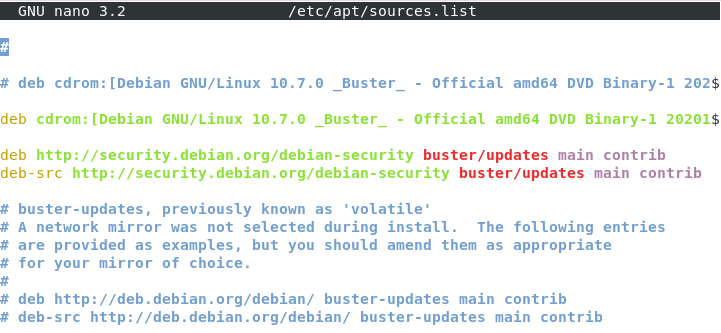
\includegraphics[scale=0.6]{sources.list}
        \end{center}
        
       \item Mettez en commentaire la ligne concernant le cdrom installé [Debian GNU/Linux...]. Sinon il vous sera demandé d'insérer le disque qui a permis l'installation comme ci-dessous.             

        \begin{center}
            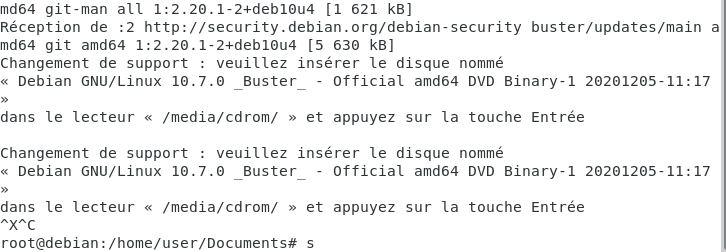
\includegraphics[scale=0.6]{cdrom}
        \end{center}
       \item Ajoutez au fichier les 4 lignes suivantes : 
       \begin{lstlisting}
deb http://deb.debian.org/debian/ buster-updates main contrib
deb-src htp://deb.debian.org/debian/ buster-updates main contrib
deb http://ftp.debian.org/debian/ buster main contrib
deb-src http://ftp.debian.org/debian/ buster main contrib
       \end{lstlisting}
    \item Cela permettra de télécharger des packets depuis les sources complètes de debian. 
    \item Enfin, sauvez le fichier et \underline{téléchargez la liste des packets à partir des sources} via la commande suivante
    \begin{lstlisting}
sudo apt-get update
    \end{lstlisting}
    \item La commande \code{apt-get update} est utilisée pour mettre à jour les informations sur les paquets disponibles à partir des dépôts de logiciels configurés sur le système. Cela permet de s'assurer que les informations sur les paquets sont à jour et que vous pouvez installer les dernières versions des logiciels disponibles.
    \item La commande \code{apt-get update} utilise les informations contenues dans le fichier \code{/etc/apt/sources.list} pour savoir où chercher les mises à jour des paquets. Ce fichier contient une liste des dépôts de logiciels où apt-get peut aller chercher les mises à jour des paquets. 
    \item Vous pouvez maintenant installer des packets tels que "git", "make" ou encore "gcc".
    \item Votre environnement de développement est maintenant prêt.
   \end{flushleft}

   \section{Privilege Escalation : Pwnkit}   		
		\subsection{Origine de la faille}   
   		\begin{flushleft}
   			\noindent Cette faille va s'intéresser à l'utilisation de la commande \textbf{pkexec} qui fait partie de la bibliothèque polkit. L'appel système pkexec est apparu en 2009 et inclus dans pratiquement toutes les distributions linux actuelles.
   			\item Cette faille de sécurité est présente depuis 12 ans et récemment mise en évidence par l'équipe de recherche Qualys en février 2022. \cite{qualys}
   			\item Cette faille permet à n’importe quel attaquant qui possède un compte sur un système linux de devenir le root du système.
            \subsection{A quoi sert la bibliothèque Polkit et en particulier l'appel système pkexec ? }
            \begin{flushleft}
                \noindent Polkit (anciennement PolicyKit) est une bibliothèque logicielle libre permettant aux applications s'exécutant avec des droits restreints d'interagir avec des services privilégiés du système. À la différence d'autres méthodes permettant une élévation des privilèges comme sudo, le processus ne se voit pas attribuer les droits super-utilisateur, ce qui permet un contrôle fin au niveau du système de ce que peuvent faire ou non les utilisateurs. \cite{policyki47:online}
                \item Polkit utilise un \textbf{démon}, également appelé service, qui s'exécute en arrière-plan sur le système et surveille les demandes d'autorisations. Lorsqu'une application tente d'exécuter une action avec des privilèges d'administrateur, le démon Polkit vérifie si l'utilisateur actuel est autorisé à exécuter cette action en utilisant les politiques définies. Si l'utilisateur est autorisé, le démon Polkit accorde temporairement les privilèges d'administrateur nécessaires à l'application pour exécuter l'action demandée.
                \item Les applications sont invitées à lui demander les droits nécessaires pour effectuer des opérations spécifiques.
                \item \textbf{En résumé}, Polkit est un système de gestion des autorisations utilisé sur les systèmes Linux pour contrôler qui peut exécuter quelles actions avec quels privilèges. Il utilise des règles de politique définies dans des fichiers de configuration pour déterminer les autorisations accordées aux utilisateurs, et un démon qui s'exécute en arrière-plan pour surveiller les demandes d'autorisations et accorder les privilèges d'administrateur nécessaires.
                \item Polkit est intégré aux distributions Ubuntu (depuis la version 8.04), Fedora (depuis la version 8), Mandriva (depuis la version 2008.1) et OpenSUSE (depuis la version 10.3).
                \subsubsection{Utilisation des "policy"}
                \begin{flushleft}
                    \noindent Les policy sont des fichiers de configuration utilisés par polkit, un système de gestion des droits d'accès qui gère les autorisations nécessaires pour exécuter des actions qui nécessitent des privilèges administratifs. Les policy contiennent des informations sur les actions qui peuvent être exécutées et les règles qui déterminent qui peut les exécuter et comment.
                    \begin{enumerate}
                        \item Les Actions sont définies dans des fichiers XML .policy situés dans \code{/usr/share/polkit-1/actions}. 
                        \begin{enumerate}
                            \item Ces fichiers peuvent être utilisés par polkit pour contrôler l'accès aux actions administratives sur le système. Vous pouvez également créer et ajouter vos propres fichiers de policy dans le répertoire /etc/polkit-1/rules.d pour personnaliser les règles d'accès sur votre système. 
                            \item Ces fichiers seront utilisés par polkit en plus des fichiers prédéfinis dans les autres répertoires, vous permettant de contrôler de manière plus fine l'accès aux actions administratives sur votre système.
                        \end{enumerate}
                        \item Les règles d'autorisation sont définies dans les fichiers .rules JavaScript. On les trouve à deux endroits : \cite{PartVMan11:online}
                        \begin{enumerate}
                            \item \code{/usr/share/polkit-1/rules.d} pour les paquets tiers peuvent utiliser (bien que peu, voire aucun, ne le fasse)
                            \item \code{/etc/polkit-1/rules.d} pour la configuration locale.
                        \end{enumerate}
                    \end{enumerate}
                \end{flushleft}
                \subsubsection{Utilisation classique de l'appel système pkexec}
                \begin{flushleft}
                    \noindent Voici un exemple d'utilisation de pkexec pour installer un nouveau paquet logiciel sur un système Linux :
                    \item \textbf{pkexec} Un programme de ligne de commande qui permet à un utilisateur d’exécuter des commandes comme un autre utilisateur. Si le programme est appelé sans argument utilisateur, la valeur par défaut est d’exécuter la commande en tant que root. Cette commande est très similaire à la commande sudo dans cet aspect. \cite{CVE2021425:online}
                    \begin{lstlisting}
$ pkexec --user <username> <command>
$ pkexec apt-get install [nom_du_paquet]
                    \end{lstlisting}
                    \item Dans cet exemple, pkexec est utilisé pour exécuter la commande \code{apt-get install} avec des privilèges d'administrateur, ce qui permet à l'utilisateur actuel d'installer un nouveau paquet logiciel sans avoir besoin de connaître le mot de passe de l'utilisateur root.
                    \item \textbf{En résumé}, l'utilisation classique de pkexec est d'exécuter des commandes en tant qu'utilisateur actuel avec des privilèges d'administrateur temporaires, afin de pouvoir effectuer des actions qui nécessitent des privilèges d'administrateur sans avoir besoin de connaître le mot de passe de l'utilisateur root.
                \end{flushleft}
                \subsubsection{Quelle est la différence entre pkexec et sudo ?}
                 \begin{flushleft}
                    \noindent Les appels système pkexec et sudo sont tous deux des outils utilisés pour exécuter des commandes avec des privilèges d'administrateur sur un système Linux. Cependant, ils fonctionnent de manières légèrement différentes.
                    \item L'appel système sudo est utilisé pour exécuter une commande en tant qu'utilisateur différent, généralement en tant qu'utilisateur root (l'utilisateur administrateur principal du système). 
                    \item Pour utiliser sudo, vous devez connaître le mot de passe de l'utilisateur root ou avoir été ajouté à la liste des utilisateurs autorisés à utiliser sudo dans le fichier de configuration \code{/etc/sudoers}.
                    \item Pkexec fait partie d'un système d'outils plus vaste appelé Polkit. Cela prend un peu de temps pour le configurer, mais une fois sur place, il donne un contrôle beaucoup plus fin.
                    \item C'est une bonne idée pour s'isoler de certains dangers et avoir l'accès complet à tout dans le système.
                    \item L'appel système pkexec est utilisé pour exécuter une commande en tant qu'utilisateur actuel, mais en accordant temporairement des privilèges d'administrateur à cette commande. 
                    \item Par exemple, si vous êtes connecté en tant qu'utilisateur foo, vous pouvez utiliser pkexec pour exécuter une commande en tant qu'utilisateur foo avec des privilèges d'administrateur. Contrairement à sudo, vous n'avez pas besoin de connaître le mot de passe de l'utilisateur root pour utiliser pkexec, mais vous devez être en mesure de fournir les informations d'authentification de votre compte utilisateur.
                \end{flushleft}
            \end{flushleft}
   		\end{flushleft}
   		\subsection{Quel est le principe de cette faille ?}
   		\begin{flushleft}
   			\noindent \textbf{pkexec} est une commande comme les autres, on peut lui passer des arguments
   			\item Mais il y a un gros problème dans la façon dont il va être implémentée, si l'argument argc est à la valeur NULL, le fonctionnement de pkexec va être déréglé. 
   			\item En manipulant des variables d'environnements et en créant des dossiers qui portent le même nom que ce qu'on va inscrire dans les variables d'environnement. Il est possible de charger un bout de code à un endroit contrôlé par l'attaquant. 
   		\end{flushleft}
   		
   		\subsection{Détails techniques sur la faille}
   		\begin{flushleft}
            \subsubsection{Ce que fait la faille}
                \begin{flushleft}
                     \noindent Pkexec de Polkit présente une vulnérabilité de corruption de mémoire conduisant à une escalade locale des privilèges
                    \item Cette vulnérabilité survient en raison d’un descripteur non sécurisé de la validation des arguments ce qui entraîne une écriture hors limite dans les paramètres envp (variables d’environnement).
                    \item Étant donné que pkexec est un binaire SUID, il s’exécute avec les privilèges root par défaut si aucun autre utilisateur ne le spécifie explicitement. 
                    \item Par conséquent, l’attaquant peut le manipuler pour exécuter du code avec des privilèges root.
                \end{flushleft}
            \subsubsection{Contexte et concepts à connaître}
            \underline{Les arguments dans la fonction main() : }
                \item On peut définir une fonction main dans les systèmes UNIX en utilisant 3 arguments.
                \begin{lstlisting}
int main(int argc, char* argv[], char *envp[])
                \end{lstlisting}
                \item \textbf{argc : } Donne le nombre d'arguments dans la ligne de commande
                \begin{itemize}
                    \item Entier qui représente la taille du tableau d’arguments,argv, qui est passé à la fonction main(). Le tableau argv est de longueur argc et se compose d’éléments commençant par argv[0] jusqu’à argv[argc-1].
                    \item Le dernier élément est un pointeur NULL, qui garantit que la liste se termine lorsqu’elle atteint sa fin.
                \end{itemize}
                \item \textbf{argv : } Est un tableau de pointeur de caractère représentant les arguments individuels fournis sur la ligne de commande.
                 \begin{itemize}
                    \item Ses éléments sont les arguments de ligne de commande transmis au programme lorsqu’il a été exécuté à partir de la ligne de commande. 
                    \item Le nom de fichier du programme en cours d’exécution est également inclus dans le tableau et constitue son premier élément.
                    \item Ainsi, par exemple, si nous voulons exécuter une commande cat, avec deux arguments supplémentaires – foo et bar – nous écrirons la commande ’cat foo bar'. Dans ce cas, argc, qui est la longueur de ce tableau, est3, et argv a trois éléments, « cat », « foo » et « bar ».
                \end{itemize}
                \item \textbf{envp : } Donne les variables d'environnement du programme. 
                \begin{itemize}
                    \item Cet argument permet à la fonction d’accéder aux variables d’environnement du programme, telles que la variable PATH, qui spécifie un ensemble de répertoires dans lesquels un programme exécutable appelé est recherché.
                \end{itemize}
                
                \begin{center}
                    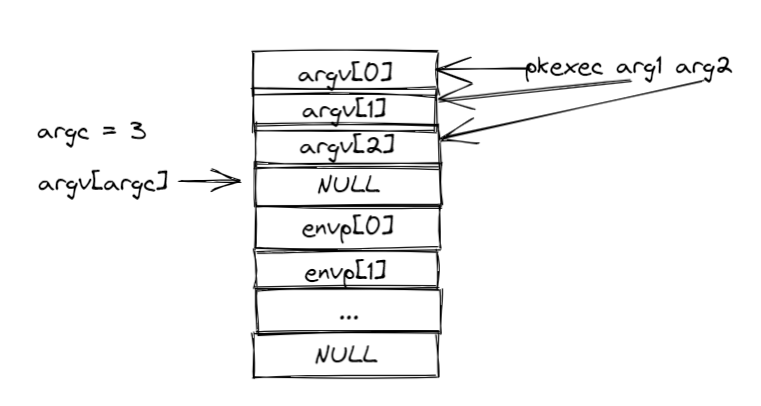
\includegraphics[scale=0.6]{main}
                \end{center}
                \newpage
            \underline{Ecriture hors-limite : }
                \item L'écriture hors limite se produit lorsqu'un programme en C essaie d'écrire des données à un emplacement mémoire en dehors de l'espace alloué pour ces données. Cela peut se produire lorsqu'un programme tente d'accéder à un tableau en dehors de ses limites définies, ou lorsqu'un programme tente d'écrire dans une zone mémoire qui n'a pas été allouée pour lui.
                \item L'écriture hors limite peut causer des problèmes graves pour un programme, tels que des plantages ou des comportements imprévisibles. Cela peut également entraîner des fuites de données sensibles ou des attaques de sécurité telles que des attaques par déni de service ou des violations de la mémoire.
                \item Pour éviter l'écriture hors limite, il est important de s'assurer que les tableaux sont correctement dimensionnés et que les limites des tableaux sont vérifiées lors de l'accès aux éléments du tableau. Il est également important de s'assurer que l'espace mémoire est correctement alloué pour toutes les données utilisées par un programme, afin d'éviter d'essayer d'écrire dans des zones mémoire non allouées.
                \item Un exemple courant est celui des tableaux de tableaux. C’est au programmeur de vérifier s’il accède à un élément qui se trouve dans la plage d’un tableau et qui ne dépasse pas sa taille.
            \item \underline{Pile d’appels :}
                 \item La pile d'appel est une structure de données utilisée par les systèmes d'exploitation pour stocker les informations sur les fonctions en cours d'exécution dans un programme. 
                 \item Lorsqu'une fonction est appelée, des informations sur cette fonction sont empilées (ajoutées) à la pile d'appel. Lorsque la fonction se termine, ces informations sont dépilées (supprimées) de la pile.
                \item Parmi les données stockées sur la pile pour la fonction main(), se trouvent les tableaux \textbf{argv} et \textbf{envp}.
                \item En fait, ils sont situés juste à côté l’un de l’autre, de sorte que la fin de argv,argv[argc], est adjacente au début de envp,envp[0].
                \begin{center}
                    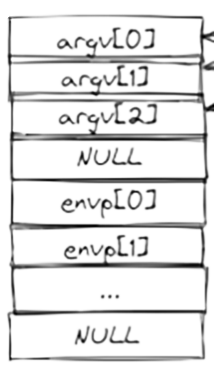
\includegraphics[scale=0.4]{pile_appel}
                \end{center}
                \newpage
            \item \underline{iconv\_open }
                \item Il s’agit d’une commande Linux qui peut être utilisée comme fonction dans le code C. 
                \item La librairie iconv\_open est une fonction de la librairie libiconv qui permet de créer un descripteur de fichier pour une conversion de caractères spécifique. 
                \item La variable d'environnement GCONV\_PATH indique l'emplacement des modules de conversion de caractères utilisés par la fonction iconv\_open, tandis que la variable gconv\_modules contient une liste des modules de conversion de caractères disponibles sur le système.
                \item En utilisant ces variables d'environnement, la fonction iconv\_open peut être utilisée pour effectuer des conversions de caractères entre différents jeux de caractères, ce qui peut être utile lors de la manipulation de texte dans des applications qui doivent gérer des données dans plusieurs encodages de caractères différents.
                \item Il est important de noter que la fonction iconv\_open ne peut pas exécuter directement de fichiers contenus dans le répertoire indiqué par la variable d'environnement GCONV\_PATH. Cette fonction ne fait que lire les modules de conversion de caractères contenus dans ce répertoire afin de pouvoir effectuer les conversions de caractères souhaitées.
                \item Toutefois, il est possible qu'un fichier malveillant puisse être introduit dans le répertoire GCONV\_PATH et utilisé par la fonction iconv\_open pour causer des problèmes sur le système. Par exemple, un fichier contenant du code malveillant pourrait être introduit dans le répertoire et utilisé par la fonction iconv\_open pour effectuer des actions nuisibles sur le système, telles que des attaques par déni de service ou la collecte de données sensibles.
                \item Il est donc important de s'assurer que le répertoire GCONV\_PATH ne contient que des modules de conversion de caractères fiables, et de surveiller régulièrement ce répertoire pour détecter tout fichier suspect. De plus, il est recommandé de mettre en place des mesures de sécurité adéquates pour protéger le système contre ce type d'attaques.
                \item Compte tenu de sa capacité à contenir des références à des bibliothèques arbitraires qui sont ensuite exécutées, la variable GCONV\_PATH était notamment connue pour faciliter les exploits d’exécution de code. 
                \item C’est pour cette raison que la variable d’environnement GCONV\_PATH est omise lors de l’exécution de programmes tels que pkexec, qui traitent de l’exécution de commandes avec des privilèges élevés temporaires.
                \begin{center}
                    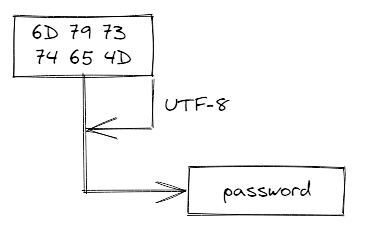
\includegraphics[scale=0.5]{iconv_open}
                \end{center}
                \cite{iconvman:online}
                \cite{gconvpath:online}
            \subsubsection{Explication ligne par ligne, pourquoi une écriture hors limite est provoquée et d'où provient la faille dans le code source de pkexec}
                \item  Vous trouverez ci-dessous une partie de la fonction main() de pkexec sur une version vulnérable à la faille, à laquelle sont donnés les arguments ci-dessus lorsque la ligne de commande est exécutée :
                \item La fonction main{} dans pkexec a une boucle for à la ligne 534, \textbf{l'initialisation de cette boucle commence par 1} jusqu'au nombre d'arguments dans la ligne de commande (argc).
                \begin{lstlisting}
534 for (n = 1; n< (guint) argc; n++)
535 {
536   if (strcmp (argv[n), "-help") = 0)
...
548     if (n >= (guint) argc)
549     {
550       usage (argc, argv);  
551       goto out;
552     }
553
554     if (opt_user != NULL)
...
564     {
565        break;
566     }
567 }
                \end{lstlisting}
                \item Ce qui veut dire que si nous passons à execve un NULL. argc serait égal à 0. La boucle sera terminée et n serait à 1.
                \item La ligne 610 argv[n] dépasse la longueur du tableau (qui est vide), ce qui signifie que le code lit au-delà des limites du tableau comme ci-dessous.
                \begin{lstlisting}
610 path = g_strdup (argv[n]);
629 if (path [0] != "/")
630 {
...
632     s = find_program_in_path (path);
...
639     argv[v] = path = s;
640  }
                \end{lstlisting}
                \item Comme décrit précédemment, la fonction main(), comme toutes les autres fonctions, peut accéder à ses arguments et variables grâce à la pile d’appels, qui les stocke de manière ordonnée. Les tableaux argv et envp sont stockés côte à côte.
                \item  Etant donné qu'argc est égal à 0 cela signifie que argv[1] pointe vers envp[0] comme illuctré ci-dessous
                \begin{center}
                    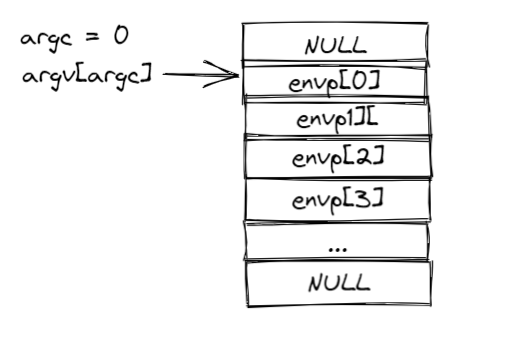
\includegraphics[scale=0.7]{ecriture environnement.png}
                \end{center}
                \item À la ligne 610, le chemin du programme à exécuter est lu hors limites à partir de argv[1] (c’est-à-dire envp[0]), et on va faire pointer cela  vers « un fichier malveillant » comme vu ci dessous.
                \begin{center}
                    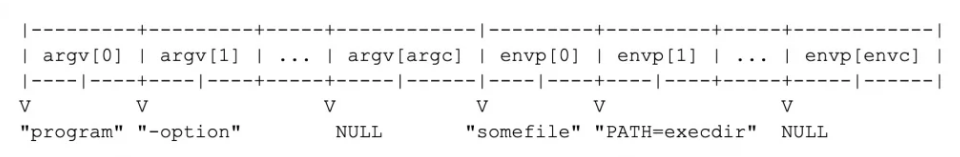
\includegraphics[scale=0.4]{image}                
                \end{center}
                \item La ligne 632 appelle la fonction g\_find\_program\_in\_path() et tente de trouver le chemin absolu du nom du programme dans le chemin, qui nous est maintenant inconnu, car il a été extrait d’une valeur lue hors limites. 
                \item Supposons qu’il existe un fichier portant le même nom que la valeur du chemin, son chemin absolu sera maintenant réécrit dans argv[n], accédant à nouveau au tableau argv au-delà de ses limites, ce qui déclenche une écriture hors limites (ligne 639).
                \item À la fin de ce flux, un emplacement mémoire en dehors du tableau argv, qui pourrait éventuellement pointer vers une chaîne qui est un nom de fichier, est remplacé par le chemin absolu du fichier.
                \item Maintenant, la question est à nouveau de savoir si nous pouvons contrôler la valeur accessible hors limites, envp[0]? 
                \item Eh bien, oui, envp[0] contient la première variable d’environnement qui est passée à pkexec lors de son exécution. 
                \item De plus, nous pouvons contrôler les variables d’environnement que nous voulons transmettre à pkexec lorsque nous l’exécutons. 
                \item \textbf{Ce qui signifie qu'envp[0] est sous notre contrôle.}
                \newpage
                \subsubsection{Ajout du code malicieux via notre environnement contrôlé}
                \item \underline{Utilisation de notre Pile d'appel}
                     \item Maintenant, appelons pkexec avec les conditions suivantes:
                     \begin{enumerate}
                         \item Nous allons définir sa liste d’arguments sur un tableau vide \{NULL\}
                         \item Nous allons définir sa liste de variables d’environnement sur \{"unfichier »,"PATH=execdir »,NULL\}
                         \item Nous allons créer un fichier exécutable dans le répertoire execdir, situé dans notre répertoire de travail actuel.
                     \end{enumerate}
                 \begin{center}
                    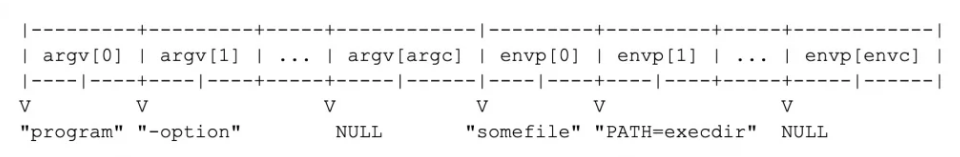
\includegraphics[scale=0.4]{image} \cite{CVE2021425:online}
                 \end{center}
                \item En d'autres termes, cette écriture hors limites nous permet de réintroduire une variable d’environnement « non sécurisée » dans l'environnement de "pkexec".
                \item Cela définit la variable d’environnement PATH pour contenir une référence au répertoire execdir. 
                \item La fonction main() va maintenant lire envp[0], qui est « unfichier », et essayer de trouver le chemin absolu de celui-ci dans le répertoire courant. 
                \item Il le trouvera, comme nous l’avons créé :  \code{/execdir/unfichier}. Enfin, il écrasera envp[0] avec le chemin absolu execdir/unfichier.
            \item \underline{Utilisation de GCONV\_PATH}
            \item GCONV\_PATH utilise la fonction iconv\_open pour exécuter le fichier exécutable répertorié dans la variable d’environnement GCONV\_PATH.
            \item Malheureusement pour nous, le répertoire GCONV\_PATH est omis de l’environnement de pkexec lors de son exécution, en raison de ses problèmes de sécurité connus expliqués plus tôt.
            \item Mais maintenant, ayant le contrôle sur envp[0], il est possible d'insérer GCONV\_PATH dans l'environnement de pkexec. Voici comment faire.
            \begin{enumerate}
                \item Nous allons définir sa liste d’arguments sur un tableau vide \{NULL\}
                \item Nous allons définir sa liste de variables d’environnement sur \{"exploit", " PATH=GCONV\_PATH=. ", NULL\}
                \item Nous allons créer un répertoire appelé GCONV\_PATH=.
                \item Nous allons créer un exploit de fichier exécutable, situé sous CONV\_PATH=. , de sorte que le chemin d’accès du fichier soit GCONV\_PATH=./exploit.
                \item Ce fichier contiendra un code simple qui exécute un shell sous les privilèges root.
            \end{enumerate}
            \begin{center}
                \includegraphics[scale=0.4]{pile d'exécution GCONV_PATH} \cite{CVE2021425:online}
            \end{center}
            \item Cela définit la variable d’environnement PATH pour qu’elle contienne une référence à au répertoire GCONV\_PATH=. 
            \item La fonction main() va maintenant lire envp[0], qui est « exploit », et essayer de trouver le chemin absolu de celui-ci dans la liste des répertoires PATH. 
            \item Il le trouvera, car nous l’avons créé sous le répertoire GCONV\_PATH=. 
            \item Enfin, il écrasera envp[0] avec le chemin absolu de GCONV\_PATH=./exploit.
            \item Nous avons maintenant introduit la variable d’environnement GCONV\_PATH exploitable dans l’environnement de pkexec. 
            \item La dernière chose à faire est de déclencher d’une manière ou d’une autre iconv\_open et de l’utiliser le répertoire GCONV\_PATH pour charger et exécuter notre fichier malveillant.
            \item \underline{Exploitation de la fonctionnalité de validation des entrées de pkexec}
            \item Pour cela pkexec dispose de beaucoup de conditions pour valider l'entrée utilisateur.
            \item Lorsqu’il rencontre une syntaxe incorrecte ou des valeurs non valides dans les arguments de ligne de commande qui lui sont transmis, ou dans les variables d’environnement qui lui sont données, il imprime un message d’erreur indicatif à l’aide de la fonction g\_printerr() de Glib (une bibliothèque libre qui peut notamment gérer les erreurs d'appels dans notre cas).
            \item Cette fonction affiche par default les messages en codage UTF-8. Dans notre cas, la variable d'environnement CHARSET n'est pas en UTF-8. C'est maintenant que nous allons utiliser la fonction iconv\_open décrite plus tôt pour convertir la sortie UTF-8 en UTF-16.
            \item La fonction va rechercher le fichier descripteur de conversion qui sera répertorié alors dans la variable d'environnement CONV\_PATH.
            \item C'est de cette manière que nous allons forcer pkexec à exécuter notre fichier malveillant répertorié sous le répertoire GCONV\_PATH.


            \subsubsection{En résumé : }
            \item Nous allons appeler pkexec avec les conditions suivantes
            \begin{enumerate}
                \item Définir sa liste d'argument sur un tableau vide
                \item Définir sa liste de variables d'environnement sur \{"exploit", "PATH=GCONV\_PATH=.", "SHELL=/not/in/etc/shells", "CHARSET=NOT\_UTF8", NULL\}
                \item Nous allons créer un répertoire GCONV\_PATH=.
                \item Nous allons créer un exploit de fichier exécutable, situé sous le répertoire GCONV\_PATH, de sorte que le chemin d'accès de GCONV\_PATH soit GCONV\_PATH=./exploit
                \item Ce fichier contiendra un code simple qui exécute un shell sous les privilèges root.
            \end{enumerate}
            \begin{center}
                    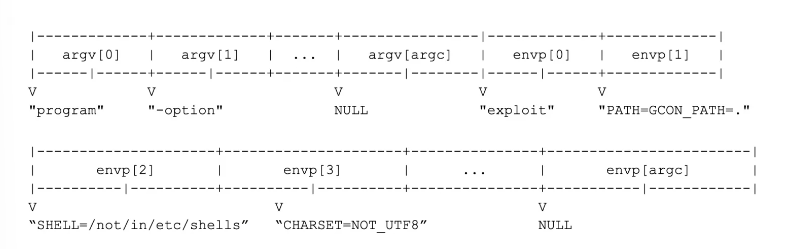
\includegraphics[scale=0.5]{pile d'appel programme final} 
            \end{center}
            \item pkexec va accéder à envp[0] et comme vu au dessus, va aller au chemin absolu de GCONV\_PATH=./exploit, où se trouve notre fichier malveillant et le réécrire dans envp[0].
            \item Ensuite il procédera à la validation des variables d'environnement que nous avons fournies. Une par une jusqu'à arriver à celle située dans envp[2].
            \item Comme il ne remplis par les conditions d'une valeur de chemin d'accès au SHELL valide. Il va affichera une erreur à l'aide de la fonction g\_printerr(). Ce qui aura pour conséquence de vérifier la variable d'environnement CHARSET, que nous avons renseignée avec la valeur "NOT\_UTF8". Comme il ne s'agit pas d'un codage UTF-8 il appelera iconv\_open() pour l'aider à convertir l'encodage du message d'erreur à la valeur "NOT\_UTF-8".
            \item La fonction iconv\_open() fera référence au fichier de conversion située alors dans la variable d'environnement GCONV\_PATH qui contient notre fichier d'exploitation malveillant. iconv\_open charge et exécute l'exploit et nous voilà sur un shell disposant des droits administrateur.

    \end{flushleft}
       \newpage

   		\subsection{Démonstration}
			\subsubsection{Fonction main()} 
			\lstinputlisting{Code/main}
             \begin{flushleft}
                \noindent Ce code déclare deux tableaux de chaînes de caractères : a\_argv et a\_envp. 
                \item Le tableau a\_argv est initialisé avec un élément NULL, tandis que le tableau a\_envp est initialisé avec une liste d'environnements.
                \begin{itemsize}
                    \item Le tableau a\_argv est utilisé pour stocker les arguments passés à une fonction ou à un programme. Dans ce cas, a\_argv est initialisé avec un seul élément NULL, ce qui signifie qu'il ne contient aucun argument.
                    \item Le tableau a\_envp est utilisé pour stocker les variables d'environnement d'un programme. Dans ce cas, a\_envp est initialisé avec une liste de variables d'environnement, notamment exploit, PATH, GCONV\_PATH, CHARSET, et SHELL. 
                \end{itemsize}
                \item Ces variables d'environnement peuvent être utilisées par un programme pour configurer son environnement d'exécution. 
                \item La variable PATH spécifie le chemins où le programme peut rechercher les commandes exécutables, tandis que la variable SHELL peut être utilisée pour spécifier le shell par défaut utilisé par le programme. Dans notre cas on spécifie un SHELL non valide pour que g\_printerr(). 
                \begin{itemize}
                     \item Comme on va spécifier que ce n'est pas un encodage UTF-8 et que cette fonction renvoie par défault les messages en UTF-8, la fonction iconv\_open sera utilisée pour rechercher le fichier descripteur de conversion qui sera répertorié dans la variable d'environnement PATH.
                \item Ce qui aura pour effet d'exécuter notre programme contenant un shell en mode root.
                \end{itemize}
               
            \end{flushleft}
   		\subsubsection{Création du dossier GCONV\_PATH et du fichier exploit dans le PATH} 
   		\lstinputlisting{Code/gconv_path}  
            \begin{flushleft}
                \noindent Fonction qui vérifie si le répertoire \code{GCONV\_PATH=.} existe. 
                \item Si ce répertoire n'existe pas, la fonction le crée avec les permissions 0777 (lecture, écriture et exécution pour tous les utilisateurs) et crée un fichier exploit dans ce répertoire avec les mêmes permissions.
            \end{flushleft}

            \newpage
            \subsubsection{Création du dossier exploit contenant un fichier module, qui exécutera le fichier malveillant lors l'appel à g\_printerr}
            \lstinputlisting{Code/iconv_open}  
            \begin{flushleft}
                \noindent Fonction qui vérifie si le répertoire exploit existe.
                \item Si ce répertoire n'existe pas, la fonction le crée avec les permissions 0777 (lecture, écriture et exécution pour tous les utilisateurs) et crée un fichier gconv-modules dans ce répertoire. 
                \begin{itemize}
                    \item Ce fichier contient une chaîne de caractères qui indique au système que le bibliothèque partagée exploit.so est un module de conversion de caractères appelé exploit compatible avec le jeu de caractères NOT\_UTF8 (ce qu'on a défini nous même dans la variable d'environnement).
                \end{itemize}
                
            \end{flushleft}
            \subsubsection{Création du fichier malveillant contenant un code simple qui exécutera un shell avec les privilèges root}
            \lstinputlisting{Code/exploit}  
            \begin{flushleft}
                \noindent Crée un fichier exploit.c dans un répertoire exploit et y écrit un programme en C qui tente de prendre les privilèges du superutilisateur (root) en appelant la fonction setuid() et setgid(). 
                
               \item La fonction \textbf{gconv\_init} utilise les fonctions \textbf{setuid}, \textbf{seteuid}, \textbf{setgid} et \textbf{setegid} pour changer les identifiants d'utilisateur et de groupe du processus en cours d'exécution (root).
               \item La variable \textbf{a\_envp[]} contient une seule chaîne de caractères \code{PATH=/bin:/usr/bin:/sbin} qui définit le chemin de recherche des programmes à utiliser lors de l'exécution de la commande shell \code{/bin/sh}. 
               \begin{itemize}
                   \item Cela signifie que lorsque la commande shell est exécutée, les programmes situés dans les répertoires \code{"/bin", "/usr/bin" et "/sbin"} seront recherchés et exécutés si la commande demandée est trouvée dans l'un de ces répertoires. 
               \end{itemize}
               
               \item Le code utilise également la fonction "execve" pour exécuter une commande shell \code{"/bin/sh"}. La fonction "execve" remplace le processus en cours d'exécution par une nouvelle instance du shell \code{"/bin/sh"}, en lui passant les arguments et l'environnement spécifiés. \item Enfin, la fonction "gconv\_init" termine le programme en appelant "exit(0)".
                \item Une fois le programme écrit dans le fichier, la fonction compile ce fichier en un bibliothèque partagée (fichier .so) en utilisant la commande gcc.
            \end{flushleft}
            
            \newpage
            \subsubsection{Fonction qui va s'occuper de vérifier si le système est vulnérable à la faille}
            \lstinputlisting{Code/checkVuln}  
            \begin{flushleft}
                \noindent Fonction qui vérifie si le système est vulnérable à l'exploit en utilisant un processus enfant.
                \item Si pkexec renvoie la chaîne de caractères "pkexec --version" au début de son output, cela signifie que le système n'est pas vulnérable à l'exploit. Sinon, cela signifie que le système est vulnérable.
            \end{flushleft}
            
            \newpage
			\subsubsection{Le script qui permet d'exécuter le programme et d'effectuer une Demo de la faille} 
			\lstinputlisting{../Code/PwnKit/Demo}  
   
		\subsection{Comment a été corrigée cette faille}
            \begin{flushleft}
                \noindent Cette faille a été corrigée dans la version 0.105 de pkexec.
                \item Ont été ajouté à plusieurs endroits du code source de pkexec, des moyens de vérifier que le nombre d'élements entré dans la commande est supérieur à 1. Si ce n'est pas le cas, sortir du programme. 
                \item Ce qui fera sortir du programme tout utilisateur malveillant tendant d'exécuter pkexec en lui donnant NULL comme liste d'arguments et ainsi exécuter une faille de dépassement de mémoire. \cite{pkexeclo25:online} 
                \item Il n'est donc plus possible de réaliser un dépassement du mémoire ce qui amenait à cette faille de sécurité.
                \begin{center}
                    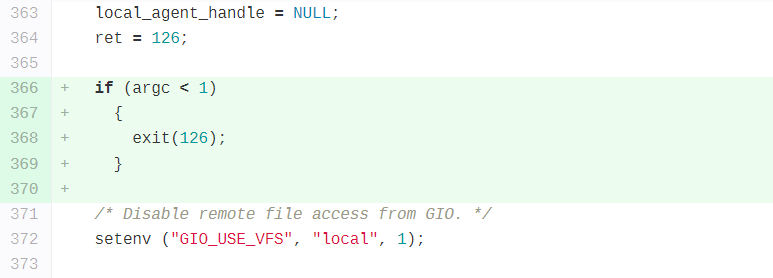
\includegraphics[scale=0.5]{verifargcsize}
                    \cite{securitytrack:online}
                \end{center}
                \item Il y a maintenant également une vérification que argv[n] doit être différent de NULL.
                \begin{center}
                    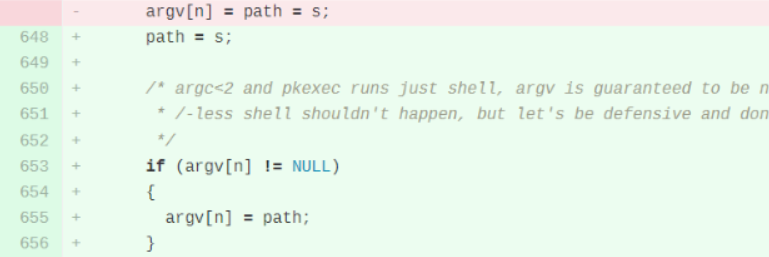
\includegraphics[scale=0.5]{verifisnull}
                    \cite{securitytrack:online}
                \end{center}
            \end{flushleft}
            
            \subsection{Comment corriger cette faille si il n'est pas possible d'ugrade la version de pkexec ?}
            \begin{flushleft}
                \noindent Si aucun correctif n’est disponible pour votre système d’exploitation, vous pouvez supprimer le bit SUID de pkexec à titre d’atténuation temporaire.
                \begin{lstlisting}
chmod 0755 /usr/bin/pkexec
                \end{lstlisting}
            \end{flushleft}
            \subsection{Est-il possible de vérifier les preuves d’exploitation?}
            \begin{flushleft}
                \noindent Oui, cette technique d’exploitation laisse par default des traces dans les logs (soit « La valeur de la variable SHELL n’a pas trouvé le fichier /etc/shells » soit « La valeur de la variable d’environnement [...] contient du contenu suspect »). 
                \item Cependant, veuillez noter que cette vulnérabilité est également exploitable sans laisser de traces dans les logs étant donné que l'attaquant dispose alors des permissions root sur le système.
            \end{flushleft}
    \newpage
   \section{Modifier le mot de passe administrateur sans le connaître}
        \subsection{Démonstration : GRUB}
        \begin{enumerate}
        	\item \textbf{Eteindre le pc} et après avoir rallumé l'ordinateur, ouvrir les options avancées et \textbf{ouvrir Grub}. Il s'agit d'un programme d'ammorçage du chargement d'un système d'exploitation. C'est ce qui fait le lien entre le bios et le système d'exploitation. Avant que le système ne soit chargé ou lancé.
        	\item Entrer en mode édition via la touche 'E'. Dans le menu GRUB, recherchez la ligne du noyau commençant par linux /boot/ et ajoutez cette ligne à la fin.
        	\begin{lstlisting}
rw init = /bin/bash
        	\end{lstlisting}
        	\item Sauvegardez les changements via en appuyant sur \textbf{CTRL + X} et rebooter en mode single-user mode.
        	\item Une fois cela fait, vous pouvez modifier le mot de passe administrateur via cette la commande ci-dessous, vous n'aurez qu'à entrer le nouveau mot de passe et une autre fois pour confirmer. Il suffit de redémarrer le système et le mot de passe administrateur aura été modifié. \cite{grubchangepassword:online}
        	\begin{lstlisting}
passwd root
        	\end{lstlisting}
         \item Cela ouvrira un shell disposant des permissions root. Il s’agit d’une fonctionnalité, utilisée pour la maintenance du système: elle permet à un administrateur système de récupérer un système à partir de fichiers d’initialisation foirés ou de modifier un mot de passe oublié.
        
        \item Il y a une alternative qui est CHROOT mais qui est très similaire dans son fonctionnement, c'est également en lien avec GRUB, je ne la détaillerait pas donc pas ici.
        \end{enumerate}
   \subsection{Pourquoi ça fonctionne ainsi ? Pourquoi est-il si simple de changer le mot de passe administrateur ?} 
   \begin{flushleft}
       \noindent Il est possible de modifier le mot de passe de l'utilisateur root via GRUB sur les systèmes Linux car GRUB permet de démarrer le système en mode sans échec, ce qui offre un accès à un shell avec des privilèges d'administrateur complets. 
       \item En mode sans échec, vous pouvez exécuter des commandes qui ont des effets sur l'ensemble du système, y compris la modification du mot de passe de l'utilisateur root.
       \item Toutefois, cette méthode est également considérée comme une vulnérabilité de sécurité, car elle permet à quiconque d'accéder à la console du GRUB de changer le mot de passe de l'utilisateur root sans autorisation.
       \item Pour protéger votre système contre ce type d'attaque, il est recommandé de configurer GRUB pour demander un mot de passe avant de permettre la modification du mot de passe administrateur, j'explique cela dans la section suivante.
   \end{flushleft}

   \subsection{Comment protéger le grub pour ne plus que cette faille soit possible} 
        \subsubsection{Configurer GRUB2 pour qu'un mot de passe ne soit exigé pour les saisie de modifications} 
        \begin{enumerate}
            \item Ouvrez un terminal et exécutez la commande sudo su pour devenir superutilisateur.
            \item Exécutez la commande \code{sudo grub2-mkpasswd-pbkdf2} pour créer un mot de passe pour protéger le grub. Lorsque vous êtes invité à entrer un mot de passe, entrez le mot de passe que vous souhaitez utiliser pour protéger le grub.
            \item Lorsque le mot de passe est créé, vous verrez un message contenant une chaîne de caractères cryptés. Par exemple, si vous avez choisi le mot de passe "password" comme mot de passe pour protéger le grub, le message contiendra une chaîne de caractères cryptés comme ceci : \code{grub.pbkdf2.sha512.10000.C8B6E7E6FB...}
            \item Copiez cette chaîne de caractères.
            \item Exécutez la commande \code{sudo vi /etc/grub.d/40\_custom} pour ouvrir le fichier de configuration du grub dans l'éditeur vi. Si vous utilisez un système différent de OpenSUSE, le fichier de configuration peut se trouver dans un emplacement différent, comme /etc/grub.d/60\_custom.
            \item Ajoutez les lignes suivantes au fichier de configuration :
            \begin{lstlisting}
set superusers="root"
password_pbkdf2 root [la chaîne de caractères...]
            \end{lstlisting}
            \item Par exemple, si vous avez choisi le mot de passe "password" comme mot de passe pour protéger le grub et que la chaîne de caractères cryptés générée à l'étape 3 est \code{grub.pbkdf2.sha512.10000.C8B6E7E6FB}, les lignes que vous ajouterez au fichier de configuration ressembleront à ceci :
            \begin{lstlisting}
set superusers="root"
password_pbkdf2 root grub.pbkdf2.sha512.10000.C8B6E7E6FB
            \end{lstlisting}
            \item Enregistrez et fermez le fichier de configuration
            \item Pour appliquer les modifications, exécutez la commande sudo grub2-mkconfig -o /boot/grub2/grub.cfg pour mettre à jour le fichier de configuration du grub.
            \item Redémarrez votre système pour que les modifications prennent effet.
        \end{enumerate}
        
        \newpage
        \section{Conclusion}
        \begin{flushleft}
            \noindent En conclusion, Linux est un système d'exploitation populaire et puissant, mais comme tout autre système d'exploitation, il n'est pas exempt de failles de sécurité. Les failles de sécurité les plus courantes sur Linux incluent les failles de type "buffer overflow", qui peuvent permettre à un attaquant d'exécuter du code malveillant sur un système Linux et de prendre le contrôle du système.
            \item Dans le cas de la faille de sécurité que j'ai expliquée, son but consistait d'injecter du code malveillant dans les variables d'environnement du code permettant d'exécuter un shell avec les privilèges root.
            \item Il est également possible de modifier le mot de passe root avec le grub, ce qui peut permettre à un attaquant d'accéder au système en tant que superutilisateur et d'exécuter des commandes avec les privilèges les plus élevés. 
            \item Pour protéger votre système Linux contre les failles de sécurité, il est important de maintenir régulièrement votre système à jour en installant les dernières mises à jour de sécurité, et de suivre les meilleures pratiques de sécurité, comme la création de mots de passe forts et l'utilisation de comptes utilisateur séparés pour limiter l'accès aux fonctionnalités administratives.
            \item De tenter au maximum de fiabiliser l'OS pour qu'il ne soit pas vulnérable aux dépassements de tampon. Auditer des programmes compilés à l'aide d'outils tels que BFBTester. Je ne détaillerais pas plus que ça ce programme mais il est utile pour tester de manière pro-active des programmes et vérifier que ceux-ci ne provoquent pas de dépassements de mémoire.
            \item Il faut également faire attention à protéger sa machine contre les attaques physiques. Si rien n'a été fait pour sécuriser son GRUB et que l'intégralité du disque n'a pas été crypté. Un attaquant peut de manière simple obtenir l'accès root et faire n'importe quoi sur la machine.
        \end{flushleft}

        \newpage
        \nocite{*}
	\bibliography{bibliozq}
	\bibliographystyle{plain}
\end{document}
